% \documentclass[lettersize,journal]{IEEEtran}
\documentclass[journal]{IEEEtran} 
\usepackage{amsmath,amsfonts}
\usepackage{algorithmic}
\usepackage{array}
\usepackage[caption=false,font=normalsize,labelfont=sf,textfont=sf]{subfig}
\usepackage{textcomp}
\usepackage{stfloats}
\usepackage{url}
\usepackage{verbatim}
\usepackage{graphicx}
\usepackage{xcolor}
% \usepackage{svg}
\usepackage{geometry} % Add this line
\usepackage{cite}
\usepackage{hyperref}
\usepackage{booktabs}
\usepackage{tikz}
\usetikzlibrary{shapes.geometric, arrows.meta, positioning}

\bibliographystyle{IEEEtran}
\hyphenation{op-tical net-works semi-conduc-tor IEEE-Xplore}
\def\BibTeX{{\rm B\kern-.05em{\sc i\kern-.025em b}\kern-.08em
T\kern-.1667em\lower.7ex\hbox{E}\kern-.125emX}}
\usepackage{balance}

\begin{document}

% }
\title{Scalable Data Aggregation for Robotics: A Multiagent Knowledge Graph System }


\author{
\IEEEauthorblockN{Christopher Allred\IEEEauthorrefmark{1},  Jacob, Chandler Justice, and All the cool people too, and Mario Harper\IEEEauthorrefmark{1}\IEEEauthorrefmark{3}}\\
\IEEEauthorblockA{\IEEEauthorrefmark{1}Department of Computer Science, Utah State University\\}
\IEEEauthorblockA{\IEEEauthorrefmark{2}Computational \& Information Sciences Directorate, Army Research Lab (ARL)}
\thanks{\IEEEauthorrefmark{3}This work was supported by Utah State University and the Army Research Lab DEVCOM AEOP  Contract Number No. W9115R-15-2-0001.}
}

% \thanks{Manuscript received April 19, 2021; revised August 16, 2021.}}

% The paper headers
\markboth{Journal of Transaction on Robotics, ~Vol.~14, No.~8, June~2024}%
{Shell \MakeLowercase{\textit{et al.}}: A Sample Article Using IEEEtran.cls for IEEE Journals}

% \IEEEpubid{0000--0000/00\$00.00~\copyright~2021 IEEE}
% Remember, if you use this you must call \IEEEpubidadjcol in the second
% column for its text to clear the IEEEpubid mark.



\graphicspath{ {./images/} }
\maketitle


\begin{abstract}
This paper presents a multiagent system designed to aggregate robot data into a structured 
knowledge graph. The proposed system utilizes multiple autonomous agents, each tasked with 
collecting, processing, and integrating data from various robotic sources. The knowledge 
graph serves as a comprehensive repository, enabling efficient data retrieval, enhanced 
interoperability, and improved decision-making for robotic applications. By leveraging 
the multiagent architecture, the system ensures scalability, flexibility, and robustness 
in handling diverse and dynamic data inputs. Experimental results demonstrate the 
effectiveness of the system in constructing a coherent knowledge graph from heterogeneous 
robot datasets, paving the way for advanced robotics research and development.
\end{abstract}

\begin{IEEEkeywords}
    Reinforcement Learning, Dynamic Motions, Legged Robots, Simulation
\end{IEEEkeywords}


\section{Introduction}
This section provides an overview of the need for structured data aggregation in robotics. It discusses the importance of a knowledge graph in enhancing data retrieval, interoperability, and decision-making. The section introduces the multiagent system approach used in this paper.

\section{System Design}
The design of the proposed multiagent system is detailed in this section. It describes the multiagent architecture and the roles and responsibilities of autonomous agents in the system, including data collection, processing, and integration. The advantages of using a multiagent system, such as scalability, flexibility, and robustness, are also discussed.

\section{Knowledge Graph Construction}
This section explains how the knowledge graph is constructed from various robotic data sources. It covers the structure and format of the knowledge graph and discusses the benefits it provides for robotics applications.

\section{Experimental Setup and Results}
The experimental setup and the datasets used to evaluate the system's effectiveness are described here. The section outlines the metrics and methods used for evaluation and presents the experimental results that demonstrate the system's ability to handle heterogeneous data and construct a coherent knowledge graph.

\section{Discussion}
An analysis of the experimental results is provided in this section. It discusses the implications of the findings for robotics research and development and compares the proposed method with existing data aggregation techniques.

\section{Conclusion}
The conclusion summarizes the key contributions of the paper and suggests potential future work to enhance the system or explore new applications.

\bibliographystyle{IEEEtran}
\bibliography{references}



% import draw io diagram
\begin{figure}[!t]
    \centering
    % it eould be nice to just import the draw io diagram
    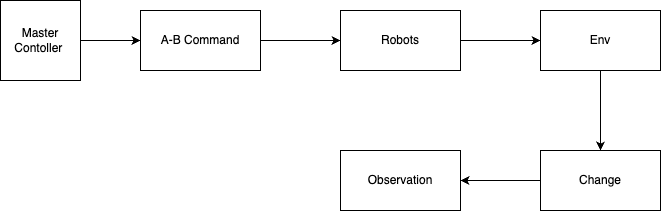
\includegraphics[width=0.5\textwidth]{images/figure.png}
    \caption{Robot Knowledge Graph System}
    \label{fig:robot_knowledge_graph}
\end{figure}


\end{document}
